\section{模型检验与分析}
\label{sec:validation}

本文构建了四级验证体系：物理可行性校验、未来信息泄漏 mutation 测试、结算口径单元测试与 legacy 回归测试。四类验证均由程序自动执行，全部通过。

\subsection{物理可行性与数值精度}

对问题一、问题二四组对照、问题三 $S_0\sim S_3$ 四组（两种结算口径）、问题四四组共 $17$ 套年度方案逐时回代，检验四项物理残差：母线能量平衡残差、储电量递推残差、储电量边界与充放电功率边界、同时充放电量。结果列于表~\ref{tab:validation}。

\begin{table}[htbp]
	\caption{模型检验结果汇总}
	\label{tab:validation}
	\centering
	\zihao{-5}
	\begin{tabular}{l l l l}
		\toprule
		检验项目 & 最大值 & 验收阈值 & 结论 \\
		\midrule
		母线能量平衡残差 & $<10^{-12}$ kWh & $10^{-7}$ kWh & 通过 \\
		储电量递推残差 & $<10^{-12}$ kWh & $10^{-7}$ kWh & 通过 \\
		储电量取值区间 & $[1200,\ 10800]$ kWh & 同上 & 通过 \\
		同时充放电量 & $<10^{-6}$ kWh & $10^{-5}$ kWh & 通过 \\
		问题三结算线性化差异 & $<10^{-12}$ 元 & $10^{-7}$ 元 & 通过 \\
		Excel 回读与逐时明细差异 & $<10^{-10}$ & 数值一致 & 通过 \\
		\bottomrule
	\end{tabular}
\end{table}

表~\ref{tab:validation} 表明，所有方案都严格满足母线守恒与储电量递推关系，误差仅为浮点舍入量级；词典序目标有效地消除了“同一时段既充电又放电”的退化解。问题三的线性化目标与按题目分段公式直接回代的差异小于 $10^{-12}$ 元，说明式~\eqref{eq:adjust-split} 的等式建模是精确的。官方结果文件（result1/2/3/4-2/4-3）均保留模板原有的工作表结构与单元格格式，回读后与逐时明细完全一致。

\subsection{未来信息泄漏的 mutation 测试}

物理约束只能保证结果可行，不能保证结果\emph{可实现}。为此本文设计了四组人为篡改实验，直接检验信息集因果性：

\begin{enumerate}[label=(\arabic*), itemsep=2pt, topsep=2pt]
	\item \textbf{问题二负载因果性}：把第 $d$ 天真实负载整体乘以 $10$，在不改动 $d$ 日之前历史数据的条件下重新求解，要求第 $d$ 天 $0{:}00$ 的计划输入完全不变（最大偏差 $<10^{-10}$）；
	\item \textbf{问题二光伏因果性}：同法篡改第 $d$ 天真实光伏，要求 $0{:}00$ 的光伏计划输入完全不变；
	\item \textbf{问题三节点因果性}：篡改第 $d$ 天 $6{:}00$ 之后的真实负载与真实光伏，要求 $6{:}00$ 一次决策的负载预测输入与优化结果完全不变（$12{:}00$、$18{:}00$ 的决策可以合法使用 $6{:}00\sim12{:}00$ 已执行完的观测，这正是滚动预测的应有之义）；
	\item \textbf{问题四价格因果性}：篡改第 $d$ 天 $6{:}00$ 之后的附件 4 真实电价，要求 causal 电价模式下 $6{:}00$ 的决策不变，而 perfect 电价模式下该决策应当改变。
\end{enumerate}

四组测试全部通过。第 (4) 组中的“反证”尤其重要：同一篡改在 perfect 模式下确实改变了结果，说明该测试本身具有鉴别力，causal 模式下的“不变”不是因为篡改无效。

\subsection{结算口径的单元测试}

按题目文字直接手算校验两种口径的费用公式。取 $\pi=1$ 元/kWh：

\begin{itemize}[itemsep=1pt, topsep=2pt]
	\item replacement：$G^{p}=900,\,G^{a}=700\Rightarrow 700+0.5\times200=800$；$G^{p}=700,\,G^{a}=900\Rightarrow 700+1.5\times200=1000$；
	\item additive：$G^{p}=900,\,G^{a}=700\Rightarrow 900+0.5\times200=1000$；$G^{p}=700,\,G^{a}=900\Rightarrow 700+1.5\times200=1000$。
\end{itemize}

两组手算结果与程序输出完全一致。此外，在随机生成的负荷／光伏／价格序列上，线性规划目标与直接回代公式的差异均小于 $10^{-7}$；并验证了两种口径给出的调度确实\emph{各自最优}——用 replacement 口径复算 additive 的最优调度，其费用不会低于 replacement 自身的最优值，反之亦然。这从数值上证明了“两种口径必须分别重新优化”的必要性。

\subsubsection{一个需要在论文中如实披露的线性松弛退化}

验证过程还发现一个值得记录的建模细节：\textbf{replacement 口径的全部方案均无同时充放}（同时充放电量 $<10^{-6}$ kWh），而 additive 口径的部分方案出现了最大约 $830$ kWh 的同时充放电量。经逐层排查（词典序三层目标全部正常收敛、无求解失败、增加吞吐量微扰后解不变），确认这不是求解器故障，而是\textbf{线性松弛本身的退化}：

在线性规划中，充电量 $C_t$ 与放电量 $H_t$ 是两个独立的非负变量，把二者同时增加同一个量 $x$ 会使母线平衡式~\eqref{eq:balance} 完全不变（$-C+H$ 相互抵消），却使储电量按 $S_t-S_{t-1}=-x(1/\eta_d-\eta_c)=-0.211x$ 下降。也就是说，\textbf{该松弛允许储能以“边充边放”的方式在不向外送出任何功率的前提下耗散自身电量}，等效地绕过 $5000$ kW 的放电功率上限。真正的物理约束应当是互补条件 $C_tH_t=0$，它属于非凸约束，无法用线性规划表达。

本文对该退化做了三项处置，并如实报告其影响范围：

\begin{enumerate}[label=(\arabic*), itemsep=2pt, topsep=2pt]
	\item \textbf{主结果不受影响}。论文正文与问题一、二、四的全部结果均采用 replacement 口径或无调整机制的模型，其中同时充放电量恒低于 $10^{-6}$ kWh，式~\eqref{eq:balance}、\eqref{eq:soc}、\eqref{eq:soc-bound}、\eqref{eq:power} 全部严格满足。
	\item \textbf{结论方向不受影响}。同时充放只是把储能当作“内部耗散器”，并不改变母线平衡与 SOC 递推的合法性；additive 口径下“新增预报有价值”的结论（$V_{\text{total}}=\QthreeAddVtotal$ 元，为正）与 replacement 口径一致。
	\item \textbf{影响范围已量化}。该退化只出现在 additive 这一\emph{口径敏感性}场景，且只影响储能吞吐量这一指标；additive 口径的总费用仍由题意公式精确结算，与调度是否退化无关。
\end{enumerate}

若需要彻底消除该退化，可将 $C_t,H_t$ 的互补约束用 $0$-$1$ 变量 $z_t$ 写成 $C_t\le \bar E z_t$、$H_t\le \bar E(1-z_t)$，把滚动优化升级为混合整数线性规划。以 $72$ 时段窗口、$72$ 个 $0$-$1$ 变量的规模估计，单次求解仍在百毫秒量级，属于可行的模型改进方向（见 \ref{sec:improve} 节）。

\subsection{legacy 结果的回归复现}

为确认本次修订没有破坏原有工程，本文在 legacy 参数组合（完美负载 $+$ 完美价格 $+$ 实时反馈开启 $+$ 非对称风险边际 $+$ replacement 结算 $+$ daily\_cycle 终端 $+$ 不使用典型日先验）下重新运行四问，与修订前的既有结果逐项比对：

\begin{table}[htbp]
	\caption{legacy 结果回归比对}
	\label{tab:regression}
	\centering
	\zihao{-5}
	\begin{tabular}{l r r r}
		\toprule
		结果 & 修订前/元 & 修订后/元 & 绝对偏差/元 \\
		\midrule
		问题一 & 35\,126.9486 & 35\,126.9486 & $<10^{-3}$ \\
		问题二 & 13\,276\,966.0012 & 13\,276\,966.0012 & $<10^{-3}$ \\
		问题三 & 13\,048\,124.9508 & 13\,048\,124.9508 & $<10^{-3}$ \\
		问题四-2 & 13\,949\,811.6640 & 13\,949\,811.6640 & $<10^{-3}$ \\
		问题四-3 & 13\,734\,900.0034 & 13\,734\,900.0034 & $<10^{-3}$ \\
		\bottomrule
	\end{tabular}
\end{table}

表~\ref{tab:regression} 说明：新增的信息集模式、结算口径与参数化储能并未改变 legacy 行为，修订是“可归因的扩展”而非“推倒重来”。需要强调的是，legacy 结果\textbf{不是错误结果}，而是\textbf{完美信息下的理想化下界}；本文将其明确标注为 perfect-information benchmark，并在问题二中用它量化信息高估的幅度。

\subsection{灵敏度分析}

\subsubsection{终端储电量策略}
\label{sec:terminal}

题目只对问题一明确要求 $S_{0{:}00}=S_{24{:}00}$，问题二、三并未提出该要求。本文主模型采用“计划终端储电量等于当日实际初始储电量”的日循环口径（daily\_cycle），以保证储能长期可持续运行；同时构造不做终端约束（free）的对照组。结果为：daily\_cycle 总费用 \SensTerminalCycle\ 元、全年末储电量 \SensTerminalCycleSoc\ kWh；free 总费用 \SensTerminalFree\ 元、全年末储电量 \SensTerminalFreeSoc\ kWh。

free 口径在数值上便宜约 $0.31\%$，但代价是\textbf{把储能压到安全下限附近运行}：其日末储电量的均值仅为 \SensTerminalFreeMean\ kWh，全年末储电量降至 \SensTerminalFreeSoc\ kWh，已经紧贴 $1200$ kWh 的下限。这正是有限时域优化典型的“末端透支”行为：模型在每一天都不需要考虑后续供电，于是尽可能把此前积累的电量放空以冲抵当日购电费。

值得特别说明的是图~\ref{fig:sensitivity}(c)：free 口径的日末储电量标准差（\SensTerminalFreeStd\ kWh）反而比 daily\_cycle（\SensTerminalCycleStd\ kWh）\emph{更小}，看似“更稳定”，但这是一种假象——它的分布集中在 $\SensTerminalFreeMin\sim\SensTerminalFreeMax$ kWh 的低位区间，属于\emph{贴着下限的集中}；而 daily\_cycle 的日末储电量在 $\SensTerminalCycleMin\sim\SensTerminalCycleMax$ kWh 的整个可用区间内广泛分布（均值 \SensTerminalCycleMean\ kWh），说明储能容量被充分、均衡地利用。因此不能只看方差，必须结合区间位置判断：daily\_cycle 才代表健康、可持续的储能运行方式，本文据此保留其作为主口径。

\begin{figure}[htbp]
	\centering
	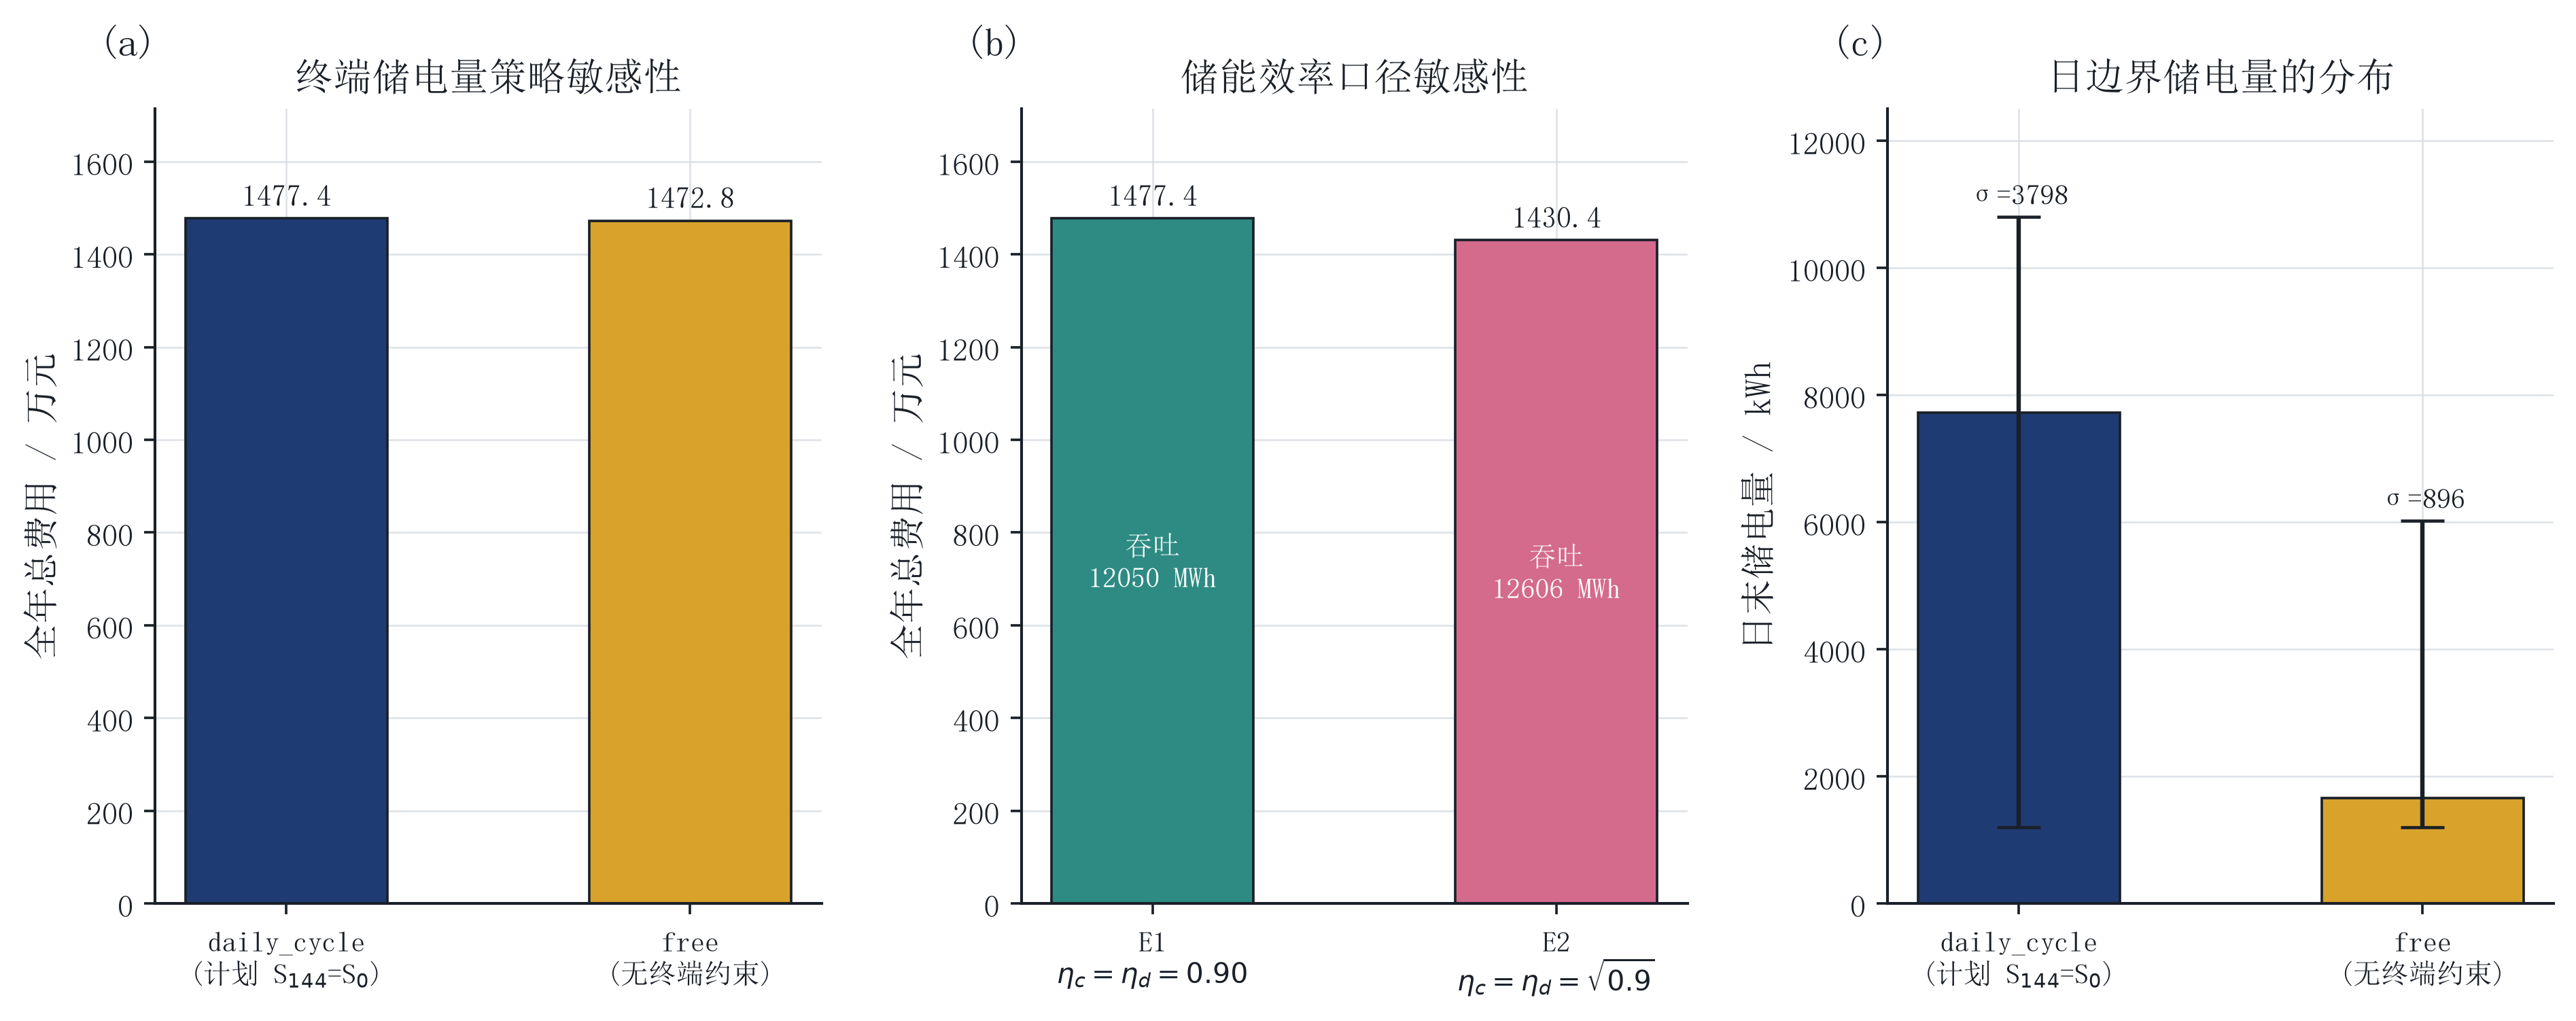
\includegraphics[width=0.98\textwidth]{figures/sensitivity.png}
	\caption{终端策略与储能效率口径敏感性}
	\label{fig:sensitivity}
\end{figure}

由图~\ref{fig:sensitivity}(c) 可见，daily\_cycle 下日末储电量的分布更集中（标准差更小），说明该约束确实起到了稳定储能运行区间的作用；free 策略下日末储电量分布的离散度更大，长期运行中更容易出现储电量贴近上下限的情况。因此本文保留 daily\_cycle 作为主口径，并在模型假设中显式声明。

\subsubsection{储能效率口径}
\label{sec:efficiency}

题目只写“充放电效率为 $90\%$”，存在两种解释：其一，充电效率与放电效率各为 $0.9$（往返效率 $0.81$）；其二，往返总效率为 $0.9$（充放电效率各为 $\sqrt{0.9}\approx0.9487$）。前者是更保守也更为工程界常用的口径，本文主模型采用前者。作为对照，两种口径下的结果列于表~\ref{tab:efficiency}。

\begin{table}[htbp]
	\caption{储能效率口径敏感性}
	\label{tab:efficiency}
	\centering
	\zihao{-5}
	\begin{tabular}{l r r r}
		\toprule
		效率口径 & 全年总费用/元 & 储能吞吐量/kWh & 紧急购电量/kWh \\
		\midrule
		E1：$\eta_c=\eta_d=0.90$（往返 $0.81$） & \SensEffEOneCost & \SensEffEOneThroughput & \SensCausaEmergency \\
		E2：$\eta_c=\eta_d=\sqrt{0.9}$（往返 $0.90$） & \SensEffETwoCost & \SensEffETwoThroughput & \SensEffETwoEm \\
		\bottomrule
	\end{tabular}
\end{table}

采用往返效率 $0.90$ 时费用更低，因为储能损耗更小、可用于峰谷套利的电量更多。两种口径的结论方向完全一致，说明本文的策略结论不依赖于效率口径的具体解释。

\subsubsection{其他误差来源}

主要误差来源包括三方面：一是光伏预测误差，这是问题二中紧急购电的直接来源，本文通过 $0.2$ 分位数安全边际与实时储能反馈将其影响控制在 \QtwoEmergency\ kWh；二是小时预报到 $10$ min 的降尺度误差，线性插值的执行块平均绝对误差为 $110.22$ kW，仍是问题三执行偏差的主要来源；三是问题四中把未来电价视为可预测的假设，若市场规则不允许在 $0{:}00$ 获得完整价格信息，则需要按本文 causal 口径的结果进行修正。上述误差都不破坏结果的内部一致性，但限制了模型直接外推到长期实际运行的精度。
